%%%%%%%%%%%%%%%%%%%%%%%%%%%%%%%%%%%%%%%%%%%%%%%%%%%
%% P3: Phenomenology of Particle Physics                         
%%
%% Author:  André Rubbia                   		 
%%
%% Figure 4.1 Geometrical setup of the double-slit experiment with electrons.
%%
%% This work is licensed under the Creative Commons Attribution 4.0 International License. 
%% To view a copy of this license, visit http://creativecommons.org/licenses/by/4.0/ or 
%% send a letter to Creative Commons, PO Box 1866, Mountain View, CA 94042, USA.
%%
%%%%%%%%%%%%%%%%%%%%%%%%%%%%%%%%%%%%%%%%%%%%%%%%%%%

\documentclass[a4paper,10pt]{article}

\usepackage[T1]{fontenc}
\usepackage[utf8]{inputenc}
\usepackage{lmodern}
\usepackage[labelfont=bf]{caption}
\usepackage{upgreek}

\usepackage{tikz}
\usepackage{pgfplots}
\pgfplotsset{compat=1.17}
\usepgfplotslibrary{ternary}
\usepgfplotslibrary{fillbetween}
\usepgfplotslibrary{external}

\def\d{\mathrm{d}}

\begin{document}

%%%%%%%%%%%%%%%%   FIGURE  %%%%%%%%%%%%%%%%%%%%%%%%%%%%%%
\begin{figure}[htb]
	\centering
	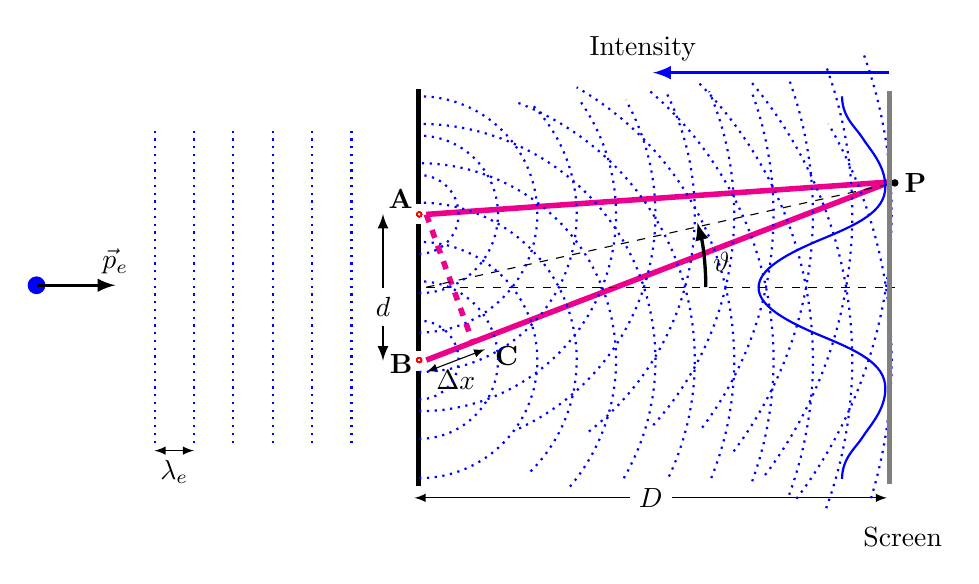
\begin{tikzpicture}[x=1mm,y=1mm,z=-0.6mm]
	\tikzstyle{axes}=[>=latex]

		\begin{scope}[axes, shift={(0,0)}]
			\draw[black] (100,0) node {Screen};
%			\draw[->] (20,31.75) node[left]  {Electron} -- +(10,0);

			\draw[black] (67,62) node {Intensity};
			\draw[->, very thick,blue] (98.3,59) -- + (180:30);

			\draw[<->,thick, color=black] (34,22.43) --
				node[fill=white,yshift=-2.5mm] {$d$} (34,41.05);
%
			\foreach \y/\dy in {6.55/14.6, 23.7/16.1, 42.3/14.6}
				\draw[ultra thick, color=black] (38.5,\y) --+(90:\dy);
% trajectories
			\draw[color=magenta, line width=2pt] (39.5,41) -- +(4:59);
			\draw[color=magenta, line width=2pt] (39.5,22.5) -- +(21:63);
			\draw[color=magenta, line width=2pt, dashed] (39.5,41) -- +(-70:17.5);
			\draw[<->,thin, color=black] (39.5,21) -- node[below] {$\Delta x$} +(21:8);
			\filldraw[color=black] (39,43) node[left] {\textbf{A}};
			\filldraw[color=black] (39,22) node[left] {\textbf{B}};
			\filldraw[color=black] (47,23) node[right] {\textbf{C}};

			\draw[<->,thin, color=black] (38,5.0) -- node[fill=white] {$D$} +(0:60);
% point P
			\filldraw[color=black] (99,45) node[right] {\textbf{P}} circle (0.4);
			\draw[color=black, thin, dashed] (39.5,31.75) -- (99,45);
			\draw[color=black, thin, dashed] (39.5,31.75) -- (99,31.75);
			\draw[->, very thick,black]  (75,31.75) arc (0:15:31.75);
			\node[color=black] at (77,35) {$\vartheta$ };

			\end{scope}
% incoming wave
			\begin{scope}[axes, shift={(5,32)}]
				\draw[blue,fill] (-15,0) circle (3pt);
				\draw[very thick,->] (-15,0)--+(0:10) node[above] {$\vec p_e$};
				\foreach \x in {0,...,5}
 				   \draw[blue,dotted,thick] (\x*5,-20)--(\x*5,20);
				\draw[<->,thin, color=black] (0,-21) -- node[below] {$\lambda_e$} +(0:5);
			\end{scope}
% Huygens waves
				\foreach \r/\min/\max in {5/-90/90, 10/-90/90,
				15/-90/90, 20/-90/45, 25/-90/35,
				30/-65/29, 35/-52/26, 40/-42/23, 45/-37/20,
				50/-37/20, 55/-37/20, 60/-37/20}
				{\draw[color=red] (38.6,41) circle (0.3);
				\draw[blue,dotted,thick,shift={(\min:\r)}] (38.6,41) arc
				(\min:\max:\r);}

				\foreach \r/\min/\max in {5/-90/90, 10/-90/90,
				15/-90/90, 20/-45/90, 25/-40/90,
				30/-30/90, 35/-25/70, 40/-22/60, 45/-20/50,
				50/-20/45, 55/-20/40, 60/-17/30}
				{\draw[color=red] (38.6,22.5) circle (0.3);
				\draw[blue,dotted,thick,shift={(\min:\r)}] (38.6,22.5) arc
				(\min:\max:\r);}

%	interference pattern on screen
			\begin{scope}[axes, shift={(81.7,31.7)}]
				\draw[-, thick, color =blue]
				(10.6,-24.3)
				..  controls (10.6,-21.6) and (12.4,-20.3)
				..
				(13.2,-19.0)
				..  controls (14.0,-17.7) and (16.1,-15.6)
				..  (16.1,-12.8)
				..  controls (16.1,-9.6) and (12.45,-8.0)
				..
				(8.0,-6.15)
				..  controls (3.05,-4.1) and (0,-2.2)
				..  (0,0)
				..  controls (0,2.2) and (3.05,4.1)
				..  (8.0,6.15)
				..  controls (12.45,8.0) and (16.1,9.6)
				..  (16.1,12.8)
				..  controls (16.1,15.6) and (14.0,17.7)
				..  (13.2,19.0)
				..  controls (12.4,20.3) and (10.6,21.6)
				..  (10.6,24.3)
				;
% screen
				\draw[ultra thick, gray] (16.6,-25) -- + (90:50);

			\end{scope}
		\end{tikzpicture}
	\caption{Geometrical setup of the double-slit experiment with electrons.}
\end{figure}
%%%%%%%%%%%%%%%%   END FIGURE  %%%%%%%%%%%%%%%%%%%%%%%%%%%
%

\end{document}
